\chapter{Design}
\label{cha:design}

This section is crucial. Describe the overall structure of your
program at a suitably high level of abstraction. For instance, UML
diagrams or informal box-and-arrow diagrams can be used to describe
program structure. Be sure to describe the MVC structure used. Note
that code listings or screenshots are not appropriate here. An
important point is how you have divided the project into modules
that different team members can work on, and how these are then
integrated. For example, you could use interfaces to describe a
clean boundary between modules, so that some team members use the
functionality provided by the interface, while another team member
implements it. Bear in mind Software Engineering principles of good
design like coherence and coupling.

\section{Release Plan}
\label{sec: release_plan}
This section outlines the proposed release plan of the project. It has been decided that the project will take the incremental approach of software development with acceptance testing taking place at each stage. The six internal releases will be implemented consecutively to bring the project to the first public release within the 10 week timeframe.

\begin{itemize}
\item \textbf{Version 0.1:} Basic player spaceship (Java shape) on screen with controls and movement.
\item \textbf{Version 0.2:} Basic shooting from the player's spaceship.
\item \textbf{Version 0.3:} Static enemies on the screen, player able to shoot the enemy and score incremented.
\item \textbf{Version 0.4:} Enemies have movement with the use of paths, are able to shoot back and collide with players.
\item \textbf{Version 0.5:} Background scrolling, enemies are spawned at regular intervals at set points using a timer.
\item \textbf{Version 0.6:} Multiplayer networking implemented.
\end{itemize} This brings the project to the first public stable release which satisfies the requirements for the assessment. It time is available certain future requirements (section \ref{sec: future_requirements}) towards the second public release.

\section{Class Design}
\label{sec: class_design}
Below shows a diagram of how the project is to be organised in terms of classes and packages (dotted lines show packages).
\begin{figure}
 \centering
 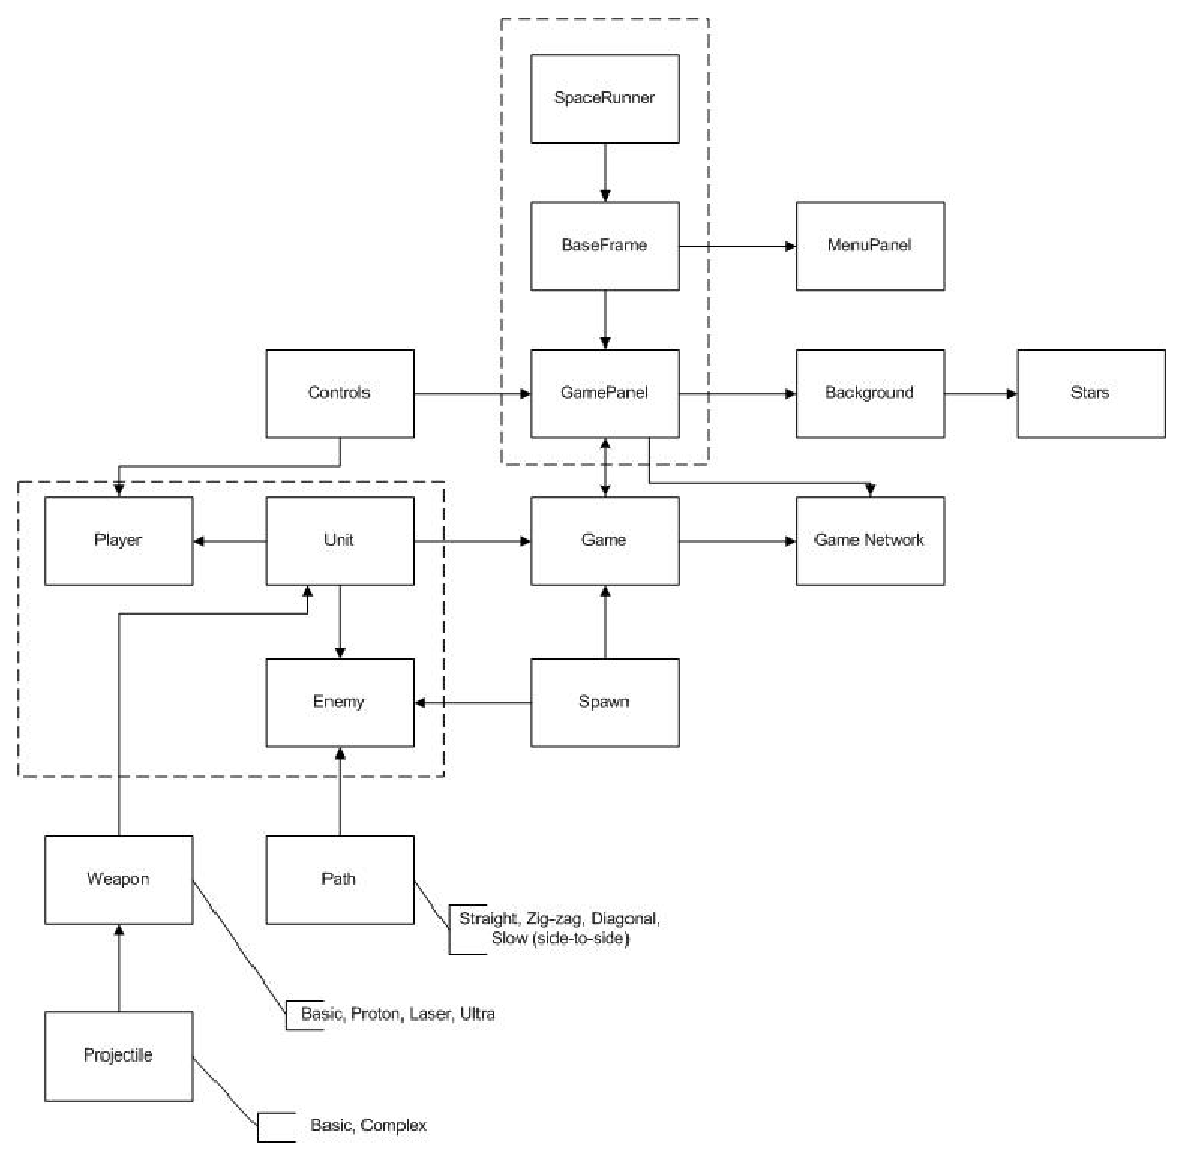
\includegraphics{class_diagram.eps}
 \caption{Proposed class diagram for the project}
 \label{fig: class_diagram}
\end{figure}

\section{Implementation}
\subsection{GUI and Controls}
The GUI was written using the standard JFrame and JPanel layout. A menu and a game panel were embedded inside the JFrame using a panel with a CardLayout. The menu and panel are part of the card layout, and can therefore be switched to very easily by referring to the name given to the CardLayout when each panel is added. There were some problems implementing a switching method to switch out the game and menu when either was required. Since the GamePanel is controlled by a timer, it is not possible to throw exceptions out. Therefore, another method was devised, by which the frame would call a method in the currently active panel to check if a `switch' flag was set. Based on this flag, the frame would change the panel that was currently being displayed, along with performing relevant actions. For example, when the menu is accessed while playing the game, the game has to be paused, and so the frame accesses a variable in the GamePanel which controls whether the game logic is progressing or not.
\subsection{Game Logic}
\subsubsection{Overview}
The game logic was written as a part of the program that could be used easily without any knowledge of the actual processing going on inside. The game logic is made up of a series of arrays, each consisting of objects that are part of the game; spawns, players, enemies and projectiles. These arrays are modified by the game in order to update the current state of the game. The arrays can be accessed by any class via getter methods, and objects can be added and removed if necessary. The logic can also perform removal of objects on command using certain pruning methods which are described later. The game logic also has methods to move all objects on the screen to new positions. The objects inside the arrays are manipulated inside the game panel using the methods of the game class. After logic has been done on the arrays, the panel then draws the objects inside the arrays.
\subsubsection{Collision detection}
The collision detection is na\"{i}ve, and done in two separate stages. Collisions of enemies with player projectiles is done first, and then collisions of enemy projectiles with the player, and enemies themselves with the player. This method is quick, and is not particularly computationally intensive given the type of game that we have written. Whether a collision actually occurs or not is defined by using a rectangular `hitbox' which surrounds the unit or projectile. If the hitboxes overlap, then the damage that the bullet carries is transmitted to the unit, and if the unit's health drops to zero or below as a result, the unit is removed from the array. The projectiles is removed from the array when it collides with a player or enemy object. Doing this gives quite a realistic feeling---it is not usual that a projectile passes through an object. However, implementing weapons that travel through units would not be problematic either, given the structure of the code. In order to avoid concurrent modification problems, enemies and projectiles that must be removed from arrays must first be stored in a secondary arraylist, which is then used to remove objects from the original array once all of the collisions have been checked.
\subsubsection{Array Pruning}
So as not to overload the memory of the computer with a huge number of objects, the arrays in the game are pruned of projectiles and enemies that are no longer within the visible area of the screen. This is done by creating a rectangle the size of the frame window, with the same coordinate space, and then, avoiding concurrent modification, removing the objects whose locations are not within the bounds of the frame rectangle. This also means that less processing is necessary during collision detection, and there are fewer objects that must be dealt with.
\subsection{Game Entities}
\subsubsection{Units}
For the units, we defined an abstract class that would contain all methods that would be necessary to access the basic information about the unit such as health. The game contains two subclasses of the unit class, player and enemy. In each of these classes, there are some parts that are specific to the requirements of those objects. For example, enemies have a method to get the value in points for destroying them, and the player class has a method to increment the score for that player. Using an abstract class meant that the subclasses already had all the necessary methods for access, and only needed some simple additional methods that were specific to the type of unit, and this saved writing quite a lot of unnecessary code. Each enemy unit moves based upon a path. Paths consist of a single equation, along with some directional variables to determine the next position of a unit based on its current position. Each time the game logic is run, this method is called with the object's current location, and returns the location that the object is due to move to next. This sort of implementation of paths allows for a robust method of control for both enemies and projectiles, and can be used to create a variety of interesting path types relatively easily, which allows for good extensibility. These paths also mean that the speed of units and projectiles can be controlled by using some sort of speed variable to increase the multiplier on the default additions to the coordinates, which would be very useful if there were to be difficulty levels added.
\subsubsection{Weapons and Projectiles}
The weapon and projectile classes are fundamental to the gameplay of the game. The weapon class is an abstract class which is intended to allow for quick addition of new weapon types into the game. Each weapon has a fire method which causes the weapon to create a new arraylist containing a number of projectiles specified by the method. This means that it is simple to add new projectiles to the game logic from quite a high position based on object orientation. Once one has a reference to a unit, it is only necessary to get the reference of the weapon, and then add the return array of the fire method to the game logic when one wants to cause weapons to fire. Each weapon has a fire rate, which is used by the logic to determine whether the weapon's fire method should be called or not. This allows for precise control of the weapons firing.

Projectiles are very simple objects which move based on paths. Each projectile object contains some data about which player it was spawned from (if it was), and details about its damage.
\subsubsection{Spawns}

\subsection{Network}
Networking is based on a client-server principle. Upon choosing the multiplayer option in the menu, the player is given a choice of hosting or joining a game. Depending on the option chosen, the game panel is initialised with server or client object which perform different tasks. When a client connects to the server via an input IP address, the server receives a reference to the client, which it then stores in a map. This map is used to get references to clients when data has to be sent to them. With a map, it is easy to send either to all clients, or choose a specific client to send data to. Client connections are dealt with by a handler, which sits in its own thread and waits for connection attempts to the server. When a connection is received, the handler adds the connection to the server's map via the interface, and the client immediately begins receiving any data from the server. Each individual client is embedded inside a class which contains methods to perform specific actions such as sending data over the network. The client and server perform interactions by first sending a string containing some information about the message that is to be sent next, and then sending the message. This method of communication is facilitated by a listener which runs in its own thread and constantly listens for commands coming in. If a command is received, a method in the socket is called to execute the request. This well structured communication method means that all communication can be handled in the correct way for that particular command. The method by which data is communicated over the network is via game state objects, which contain all the data needed by the game to run correctly; all the arrays, and boolean variables representing whether the game is running or not, along with a few others. The game state is capable of doing some processing, in order to reduce the data that is transferred over the network. A client first receives data from the server, and then runs its logic on it, moving projectiles fired by all units, and moving the player location. Each loop, the current state of the game is made into a new game state. This game state is then compared against the game state that was received from the server at the start of the loop. All objects that are the same in both game states are ignored---only new objects and the player reference are passed to the server, which reduces load on the network and also makes it easier for the server to collate the data into a single new game state which combines data from all clients which are currently connected. The server takes the new amalgamated game state, performs logic on it, and then sends it out to all clients, and the cycle continues. This method, along with the client storage method means that clients can drop in and out of the game without any wait time. In order to facilitate the transfer of objects over the network, upon object creation, each object is given a reference which will allow checking of the objects even if they are duplicated later, which is necessary for the removal of old objects.
\subsection{Graphics}
Graphics is implemented using a map stored in the game panel class. This map is initialised upon loading of the game with images from the relevant locations. Each object which must be drawn has an image reference string, which refers to the string that the image was added to the map with. When the object is drawn, the image reference is used to retrieve the image for that particular object, which is passed to the draw method of the object, which then draws it. Using this method meant that it was not necessary to pass images over the network, which would greatly slow communication due to the relatively large size of images. However, this method could, in theory, lead to the modification of the image files which are used to draw objects. In actuality, this will have no real effect on gameplay, since the size of the images are not at all considered when processing game logic.


%%% Local Variables: 
%%% mode: latex
%%% TeX-master: "report"
%%% End: 